\section{Модуль отображения логического времени на физическое}
\indent В соответствии с архитектурой, представленной ранее\todo{формулировка}, расчет выполнения операции (или набора операций) производится в логическом времени,т.~е. во времени отсчитываемом от нуля.
Данное решение обуславливает необходимость в отображении (соответствие между элементами двух множеств) логического времени на физическое, которое используется в повседневной жизни.
Одной из главных сложностей, возникающих при этом, является неоднородность рабочего времени, которая проявляется в рабочем графике (чередование интервалов рабочего и нерабочего времени), наличии выходных, перенесенных дней.
Другой сложностью является наличие в системе 'обратного расчета', при котором планирование ведется от даты 'дедлайна' (дата или время, к которому должна быть выполнена задача), что накладывает некоторые ограничения на реализацию данной компоненты.\\
% \subsection{идея}
\indent Для отображения логического времени на физическое был предложен итеративный процесс, который осуществляет 'переход' к необходимому времени путем последовательного перебора.\\
\indent Как было сказано ранее, из-за того, что рабочее время является дискретным, то мы не имеем возможности просуммировать начальную дату и значение поданного логического времени.
Это ведет к тому, что необходимо синхронизировать логическое и физическое время, и в данной компоненте это достигается путем последовательного периодического отображения конкретного логического времени на физическое (см. \ref{fig:axes}).
Это подразумевает под собой наличие двух массивов чисел или 'осей': оси логического времени, которая начинается с нуля и единица которой соответствует одной секунде (необходимости в более точном отображении нет) и оси физического времени, на которой может быть отложено любая дата физического времени, отсчет которой начинается 1 января 1970 года 00:00:00 (эпоха Unix).
Особенностью оси физического времени является наличие на ней 'выколотых' промежутков времени, в которые работа не ведется и операции не выполняются и следовательно об этих промежутках системе необходимо знать, и они передаются системе в виде структуры данных, которая далее будет называться 'конфигурацией модуля'.\\
% \subsection{Входные и выходные данные}
\indent Входными данными для модуля являются:

\begin{itemize}
	\item дата с которой необходимо начинать отсчет;
	\item логическое время, которого необходимо достигнуть;
	\item конфигурация модуля.
\end{itemize}

\indent Дата является точкой на физической оси, на которую будет отображаться нуль логической. Представляет собой количество секунд, прошедшее с начала эпохи Unix.\\
\indent Логическое время~-~количество секунд, которое должно быть отложено на логической оси. В силу дискретности\todo{неправильный термин} физической оси, каждой логической точке сопоставляется отрезок на физической оси, сопоставляется пара чисел - границ данного отрезка.\\
\indent Конфигурация модуля~-~вспомогательные данные используемые для определения модулем какие промежутки необходимо пропускать в процессе работы.
Состоит из данных о рабочем графике занятого персонала (интервалы рабочего времени), шаблонном расписании на неделю (например, суббота, воскресенье - выходные, пятница - 'короткий' день, остальные - стандартные рабочие дни) и набор информации о датах, которые являются днями-исключениями и соответствующей информацией о графике работы в данные дни.\\
% \subsection{Результат работы}
\indent Выходными данными данного модуля является пара чисел, характеризующие начало и конец отрезка которые отображаются на логическую ось в точке, значение которой равно входному логическому времени.\\

\begin{figure}[h]
	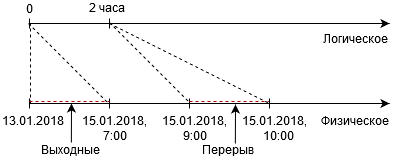
\includegraphics[width=\linewidth]{pics/scheduleAxes.png}
	\caption{Пример отображения оси логического на ось физического времени}
	\label{fig:axes}
	\centering
\end{figure}

% \subsection{Реализация}
\indent После запуска, модуль получает параметры и совершает проверку последних на корректность и непротиворечивость (например, если два дня имеют пересечения временных промежутков то они противоречивы, ведь ресурс не может работать одновременно в двух сменах) как в рамках смен одного так соседних дней.
Далее производится определение режима работы: прямой, обратный расчет или проверка времени:\todo{нужно более емкое понятие}.

\begin{itemize}
	\item прямой расчет - задается дата начала отсчета, логическое время и расчет ведется до нахождения даты окончания работ (см \ref{fig:straightCalc});
	\item обратный расчет - задается дата дедлайна, логическое время и расчет ведется до нахождения времени начала работ(см \ref{fig:reverceCalc});
	\item проверка времени - задается дата и логическое время равное нулю, что запускает оба предыдущих расчета пока не будет найдено первое ненулевое время в обоих направлениях от даты начала расчета(см \ref{fig:checkCalc}).
\end{itemize}

\begin{figure}[h]
	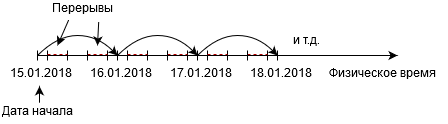
\includegraphics[width=\linewidth]{pics/scheduleStraightCalc.png}
	\caption{Схема прямого расчета}
	\label{fig:straightCalc}
	\centering
% \end{figure}
% \begin{figure}[h]
	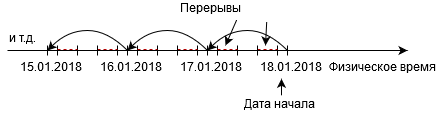
\includegraphics[width=\linewidth]{pics/scheduleReverceCalc.png}
	\caption{Схема обратного расчета}
	\label{fig:reverceCalc}
	\centering
% \end{figure}
% \begin{figure}[h]
	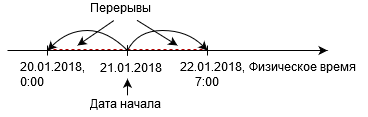
\includegraphics[width=\linewidth]{pics/scheduleCheckCalc.png}
	\caption{Схема проверки времени}
	\label{fig:checkCalc}
	\centering
\end{figure}

\indent Выбрав режим работы сбрасывается счетчик текущего логического времени до нуля и счетчик текущего физического времени до стартовой даты. Затем итеративно, пока текущее логическое время не превысит необходимое производится поиск следующей даты.
Алгоритмически, поиск даты работает следующим образом:

\begin{enumerate}
	\item[1)] определяются интервалы рабочих смен относящихся к текущему дню:
	      \begin{itemize}
		      \item при отсутствии таковых, к текущей дате прибавляется один день и затем возврат к п.1.
	      \end{itemize}
	\item[2)] отсортированные в порядке возрастания, интервалы последовательно перебираются и их длительности прибавляются к текущему логическому и физическому времёнам:
	      \begin{itemize}
		      \item при превышении текущим логическим временем необходимого, переход к п.3;
		      \item если все интервалы были просуммированны, но необходимое логическое время не превышено - переход к п.1;
	      \end{itemize}
	\item[3)] вычитается из физического времени разность текущего и необходимого логического времён, при этом сохраняя данное значение как левую (правую при обратном расчете) и продолжается расчет для выявления правой (левой) границы промежутка
\end{enumerate}

\begin{figure}[h]
	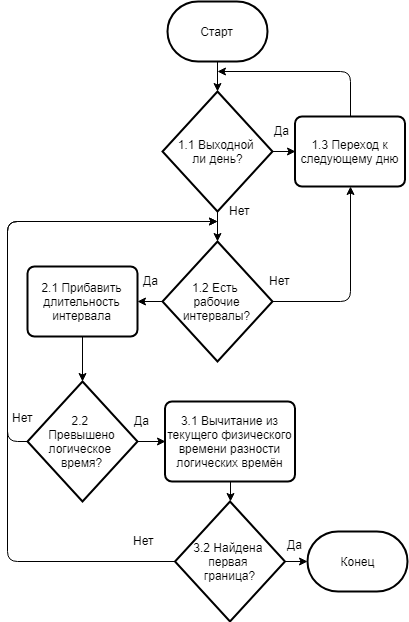
\includegraphics[width=\linewidth]{pics/scheduleSchema.png}
	\caption{Блок-схема модуля}
	\label{fig:schema}
	\centering
\end{figure}

\indent Определение интервалов рабочего времени происходит взятием даты из текущего физического времени, после чего начинается определение является ли данная дата одной из перенесенных после чего есть два варианта развития ситуации:

\begin{itemize}
	\item дата является перенесенным днем и модуль получает информацию о расписании которое нужно применить;
	\item дата не является перенесенным днем и получение информации происходит исходя из того, каким днем недели является данная дата.
\end{itemize}

\todo[inline]{пояснение трудностей}
\todo[inline]{схема трудности обратного расчета}
% \todo[inline]{Так как расчет расписания — это итеративный процесс, то в рамках разработки было выделено понятие временной линии (прямой) – это «линия» на которой для каждой точки, которая является абстрактной величиной времени выполнения операции, сопоставляются две даты соответствующие данной абстрактной величине времени с учетом расписания. Первая дата является концом данной операции, вторая – началом следующей. Данное разделение было использовано, потому как все время что между ними также относится к данной точке, а значит каждой точке, из-за непрерывности времени, соответствует бесчисленное множество точек на временной прямой, что может быть лишь ограничено двумя границами – временем начала и конца данного отрезка.}